% !TeX root = ../dokumentation.tex

\chapter{Projekt Ergebnisse}

\section{Analyse der Organisatorischen Änderungen}

\subsection{Kapazitätsschätzungen}

Zu Beginn des Projektes gab es Schwierigkeiten mit der Planung des Sprintumfangs.
Im ersten Sprint konnten vorgenommene Tickets nicht abgeschlossen werden. 
Dadurch konnte das Sprintziel nicht erreicht werden (vgl. Abbildung~\ref{fig:SKIOS-Sprint-1-Brundown}).

\begin{figure}[h]
    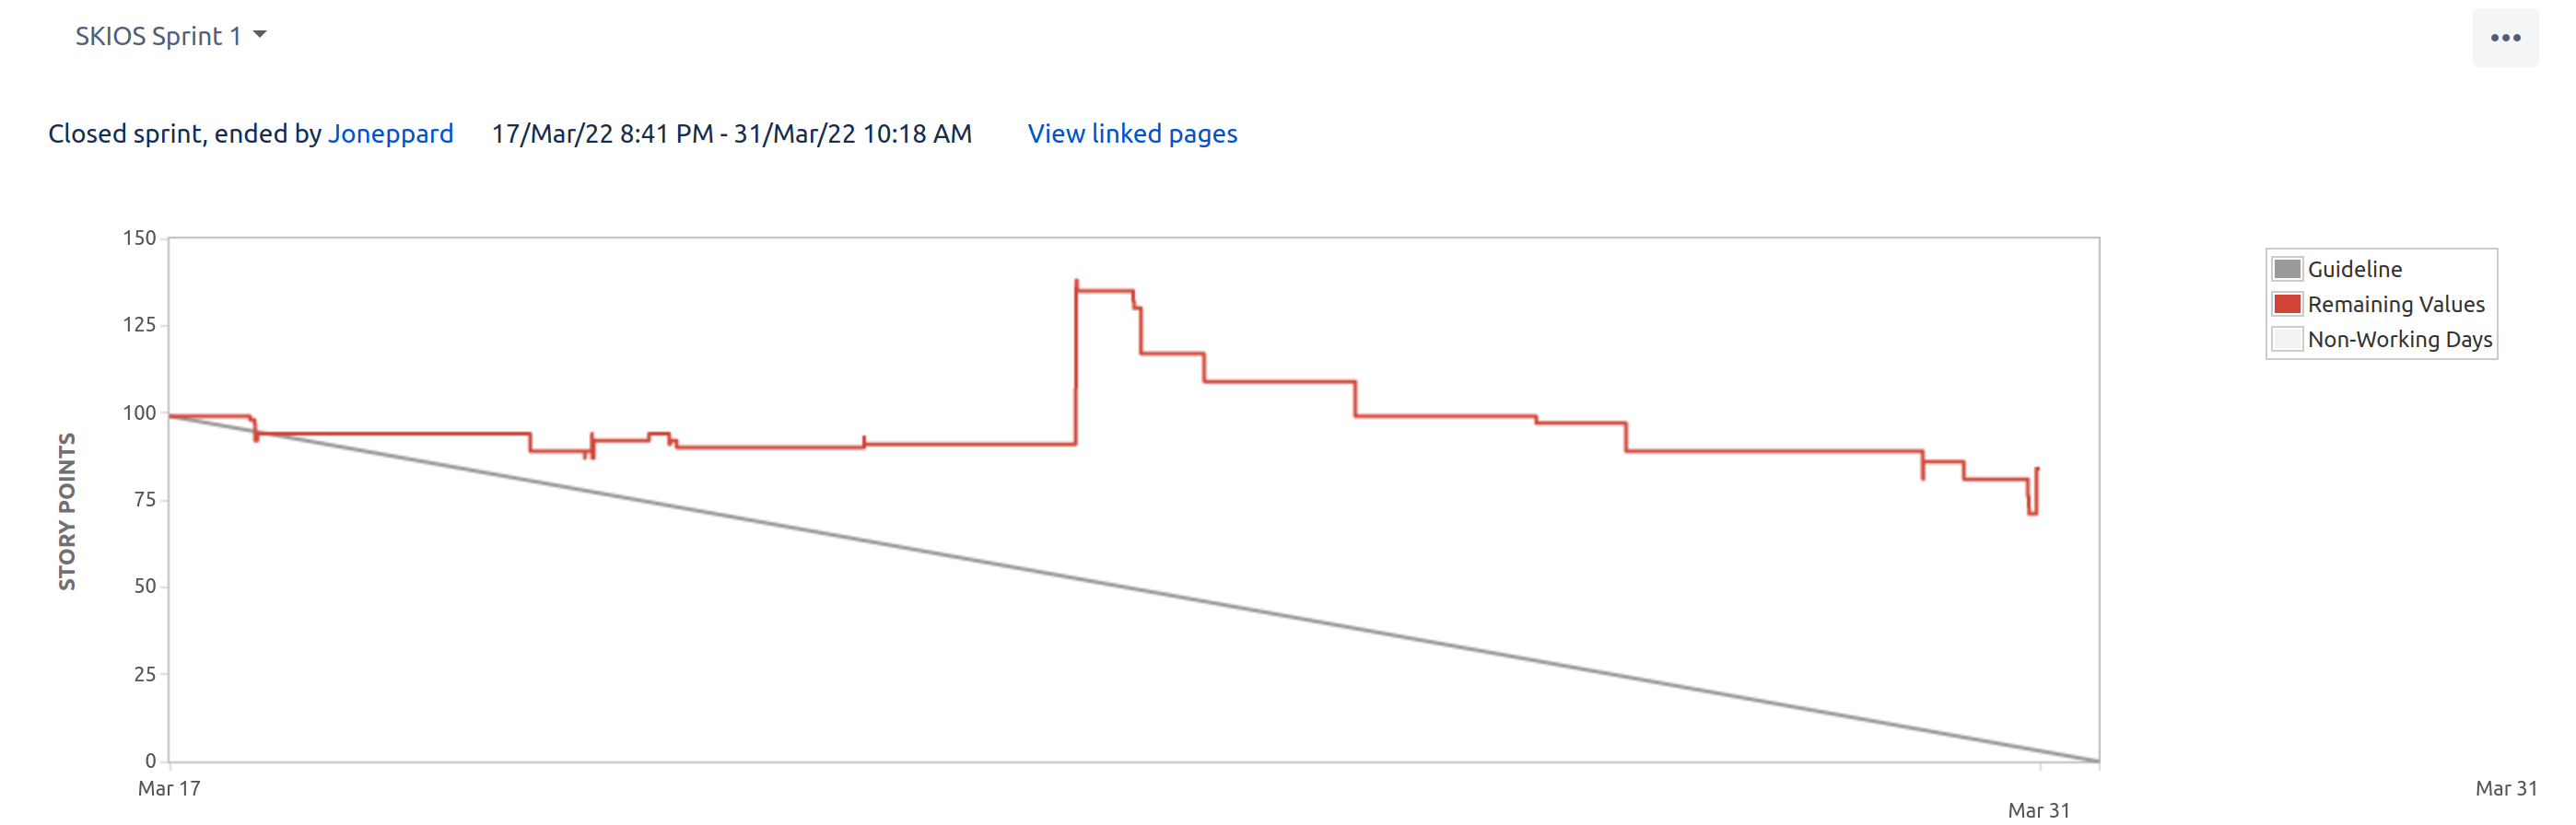
\includegraphics[width=\linewidth]{SKIOS-Sprint-1-Brundown-Diagram.png}
    \caption{Brundown-Chart zu Sprint 1}
    \label{fig:SKIOS-Sprint-1-Brundown}
\end{figure}

Unter anderem wurde in der Retrospektive daraufhin festgehalten, 
dass sich die Kapazitäten zwischen den einzelnen Teammitgliedern sehr stark unterschieden.
Für den Sprint 1 ist man davon ausgegangen, dass jedes Teammitglied 20 Storypoints im Sprint bearbeiten kann.
Damit genauer geplant werden kann, wurde im Confluence eine Seite zur Kapazitätsschätzung eingerichtet.
Dabei handelt es sich um eine Tabelle, in der jedes Teammitglied in Storypoints die eigene Kapazität einschätzen konnte.
Diese wurde wie in Abbildung~\ref{fig:Capacitytable} erstellt. 

\begin{figure}[h]
    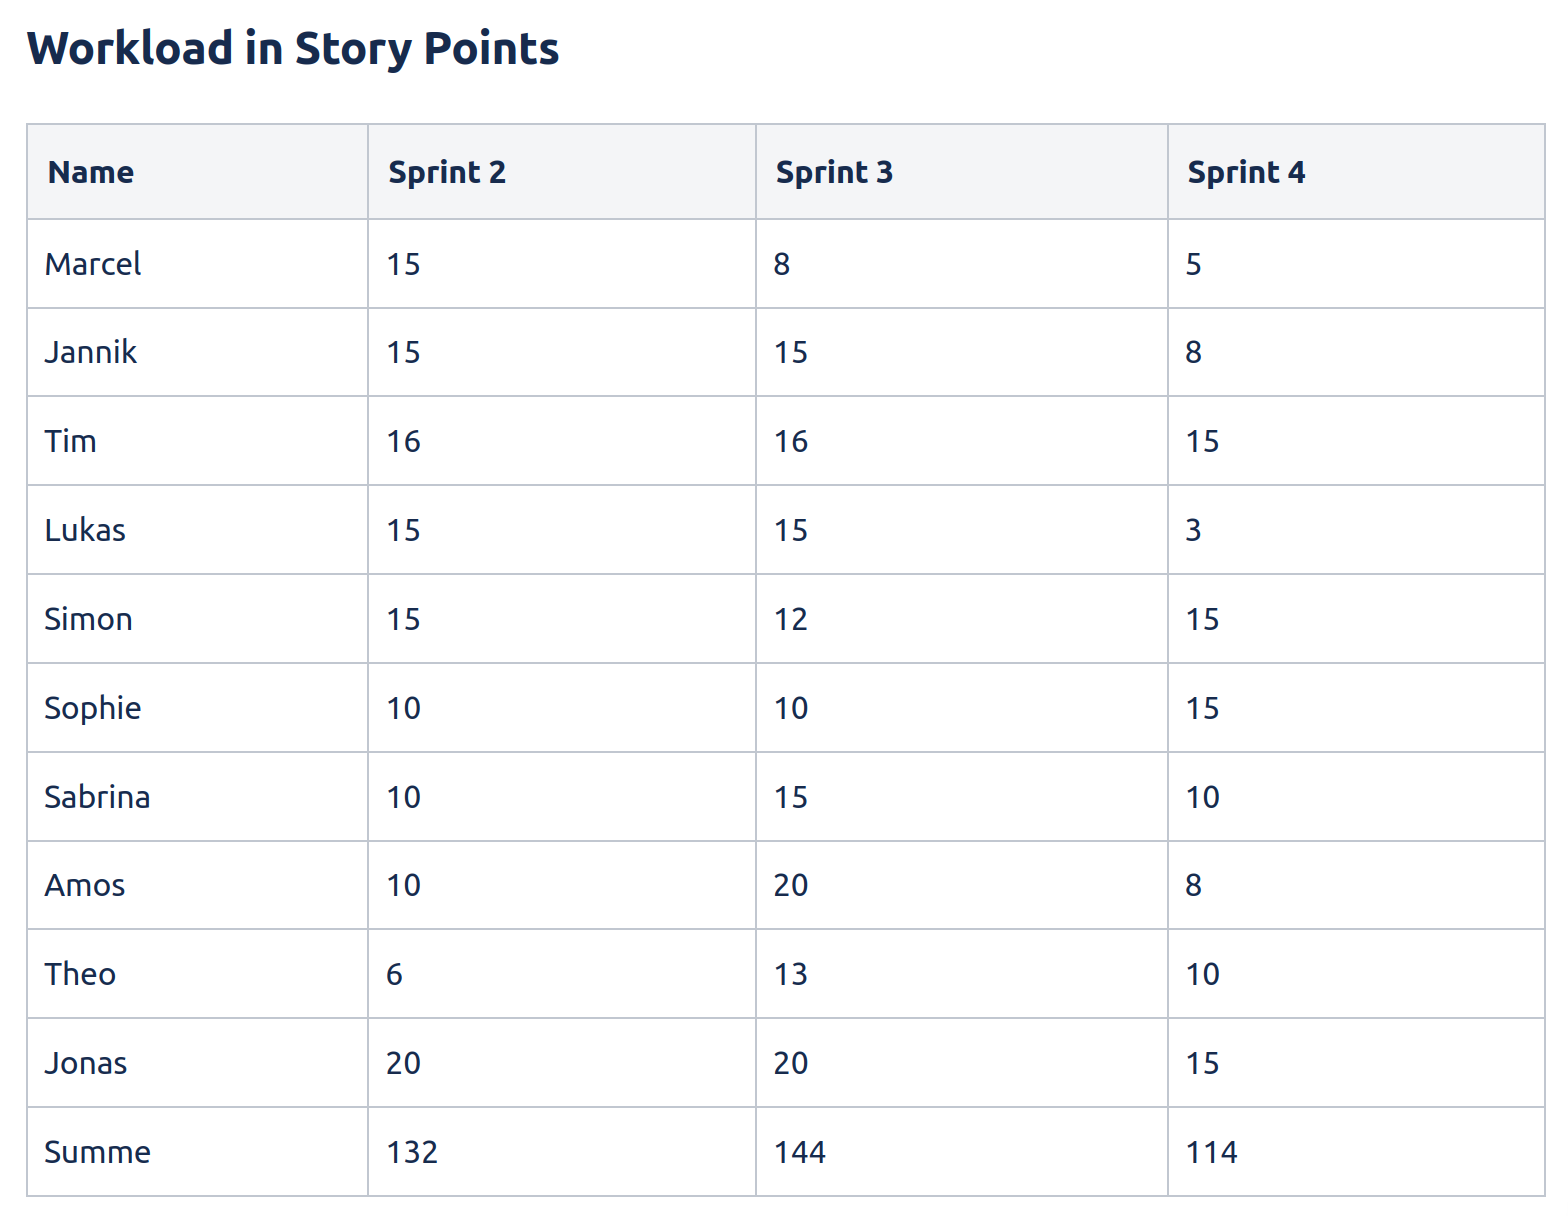
\includegraphics[width=\linewidth]{SKIOS-Capacity-Esitmates.png}
    \caption{Kapazitätschätzungen der Teammitglieder}
    \label{fig:Capacitytable}
\end{figure}

Mit einer besseren Kapazitätsschätzung konnten im nächsten Sprint, dann auch deutlich mehr vorgenommene Tickets abgeschlossen werden (vgl. Abbildung~\ref{fig:SKIOS-Sprint-2-Burndown}).
Es war möglich zumindest vorhersehbare Ereignisse, die die Kapazität einzelner stark einschränken, abzufangen.
Im dritten Sprint wurden auch die Schätzungen der eigenen Kapazität besser, wodurch dann auch das Sprintziel erreicht wurde (vgl. Abbildung~\ref{fig:SKIOS-Sprint-3-Burndown}).

\begin{figure}[H]
    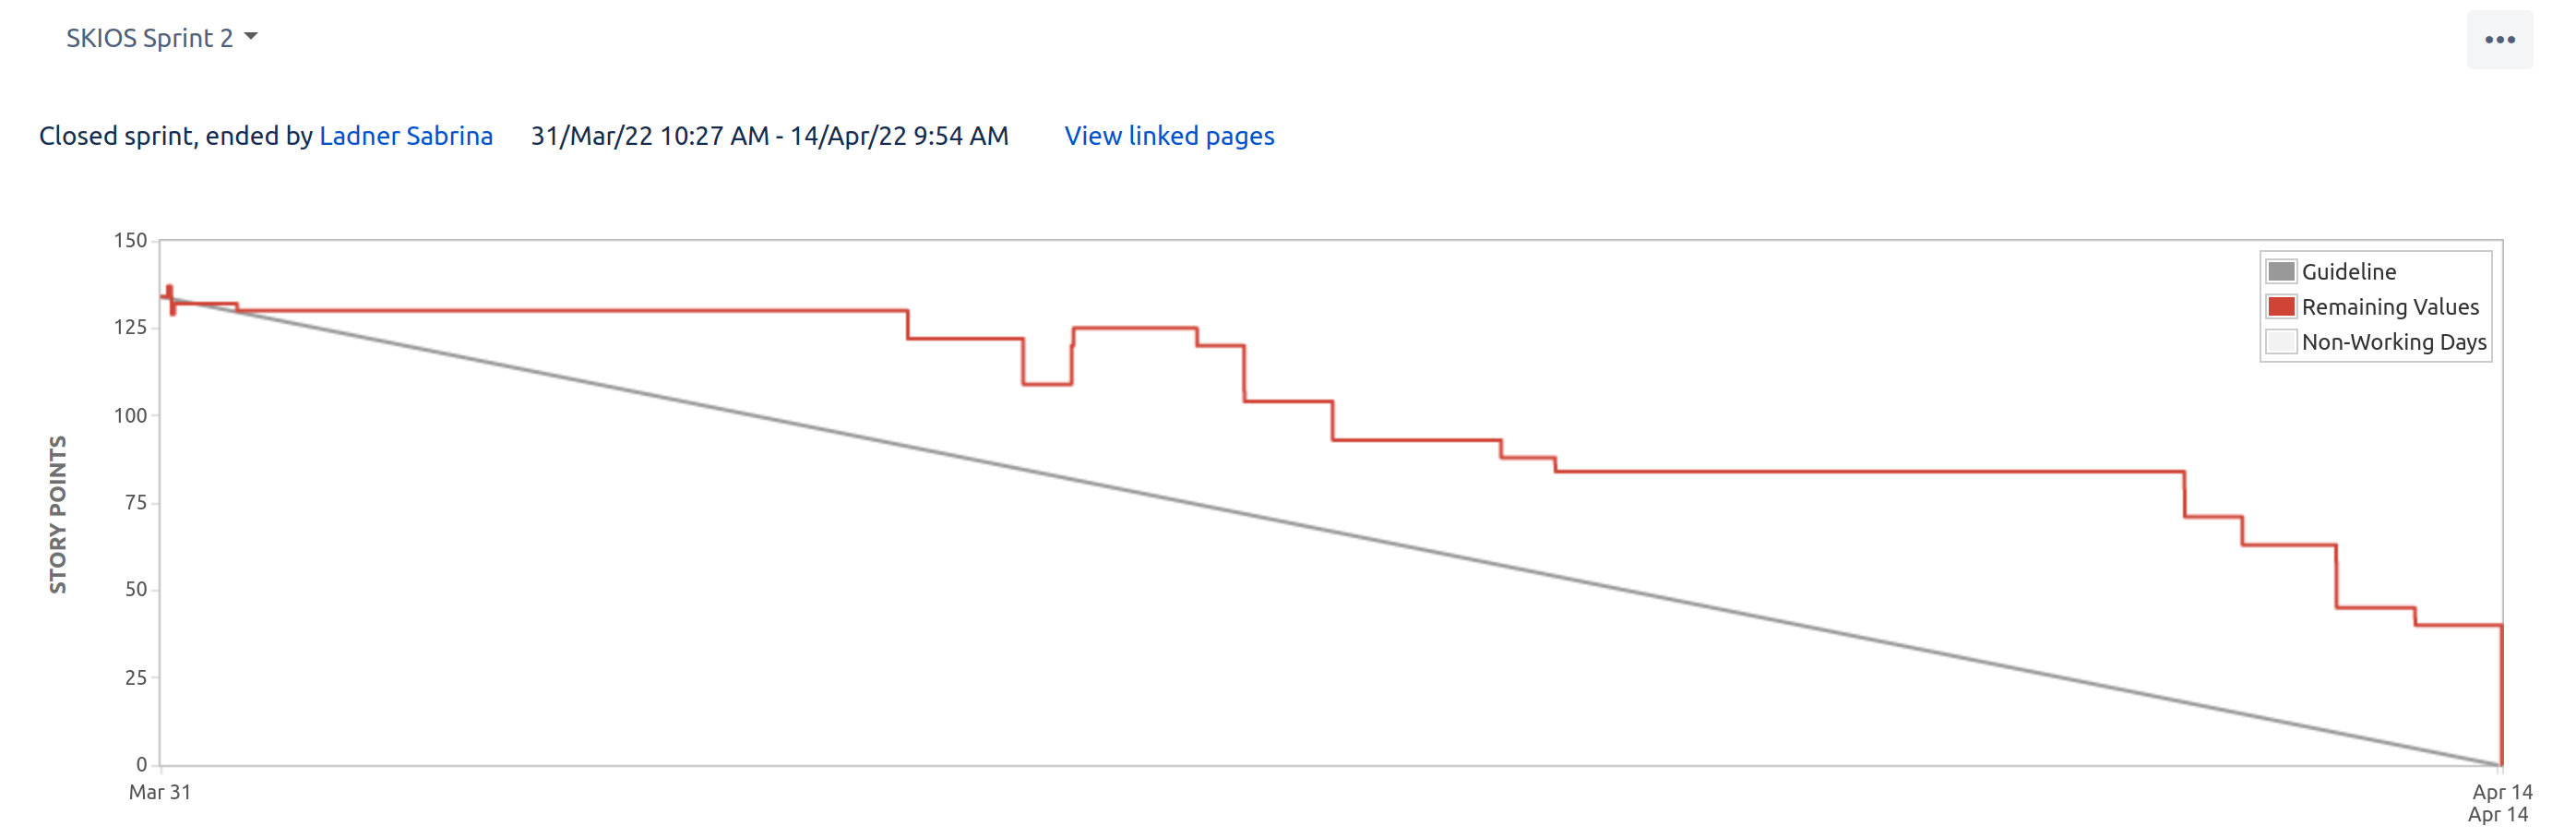
\includegraphics[width=\linewidth]{SKIOS-Sprint-2-Brundown-Diagram.png}
    \caption{Burndown-Chart zu Sprint 2}
    \label{fig:SKIOS-Sprint-2-Burndown}
\end{figure}

\begin{figure}
    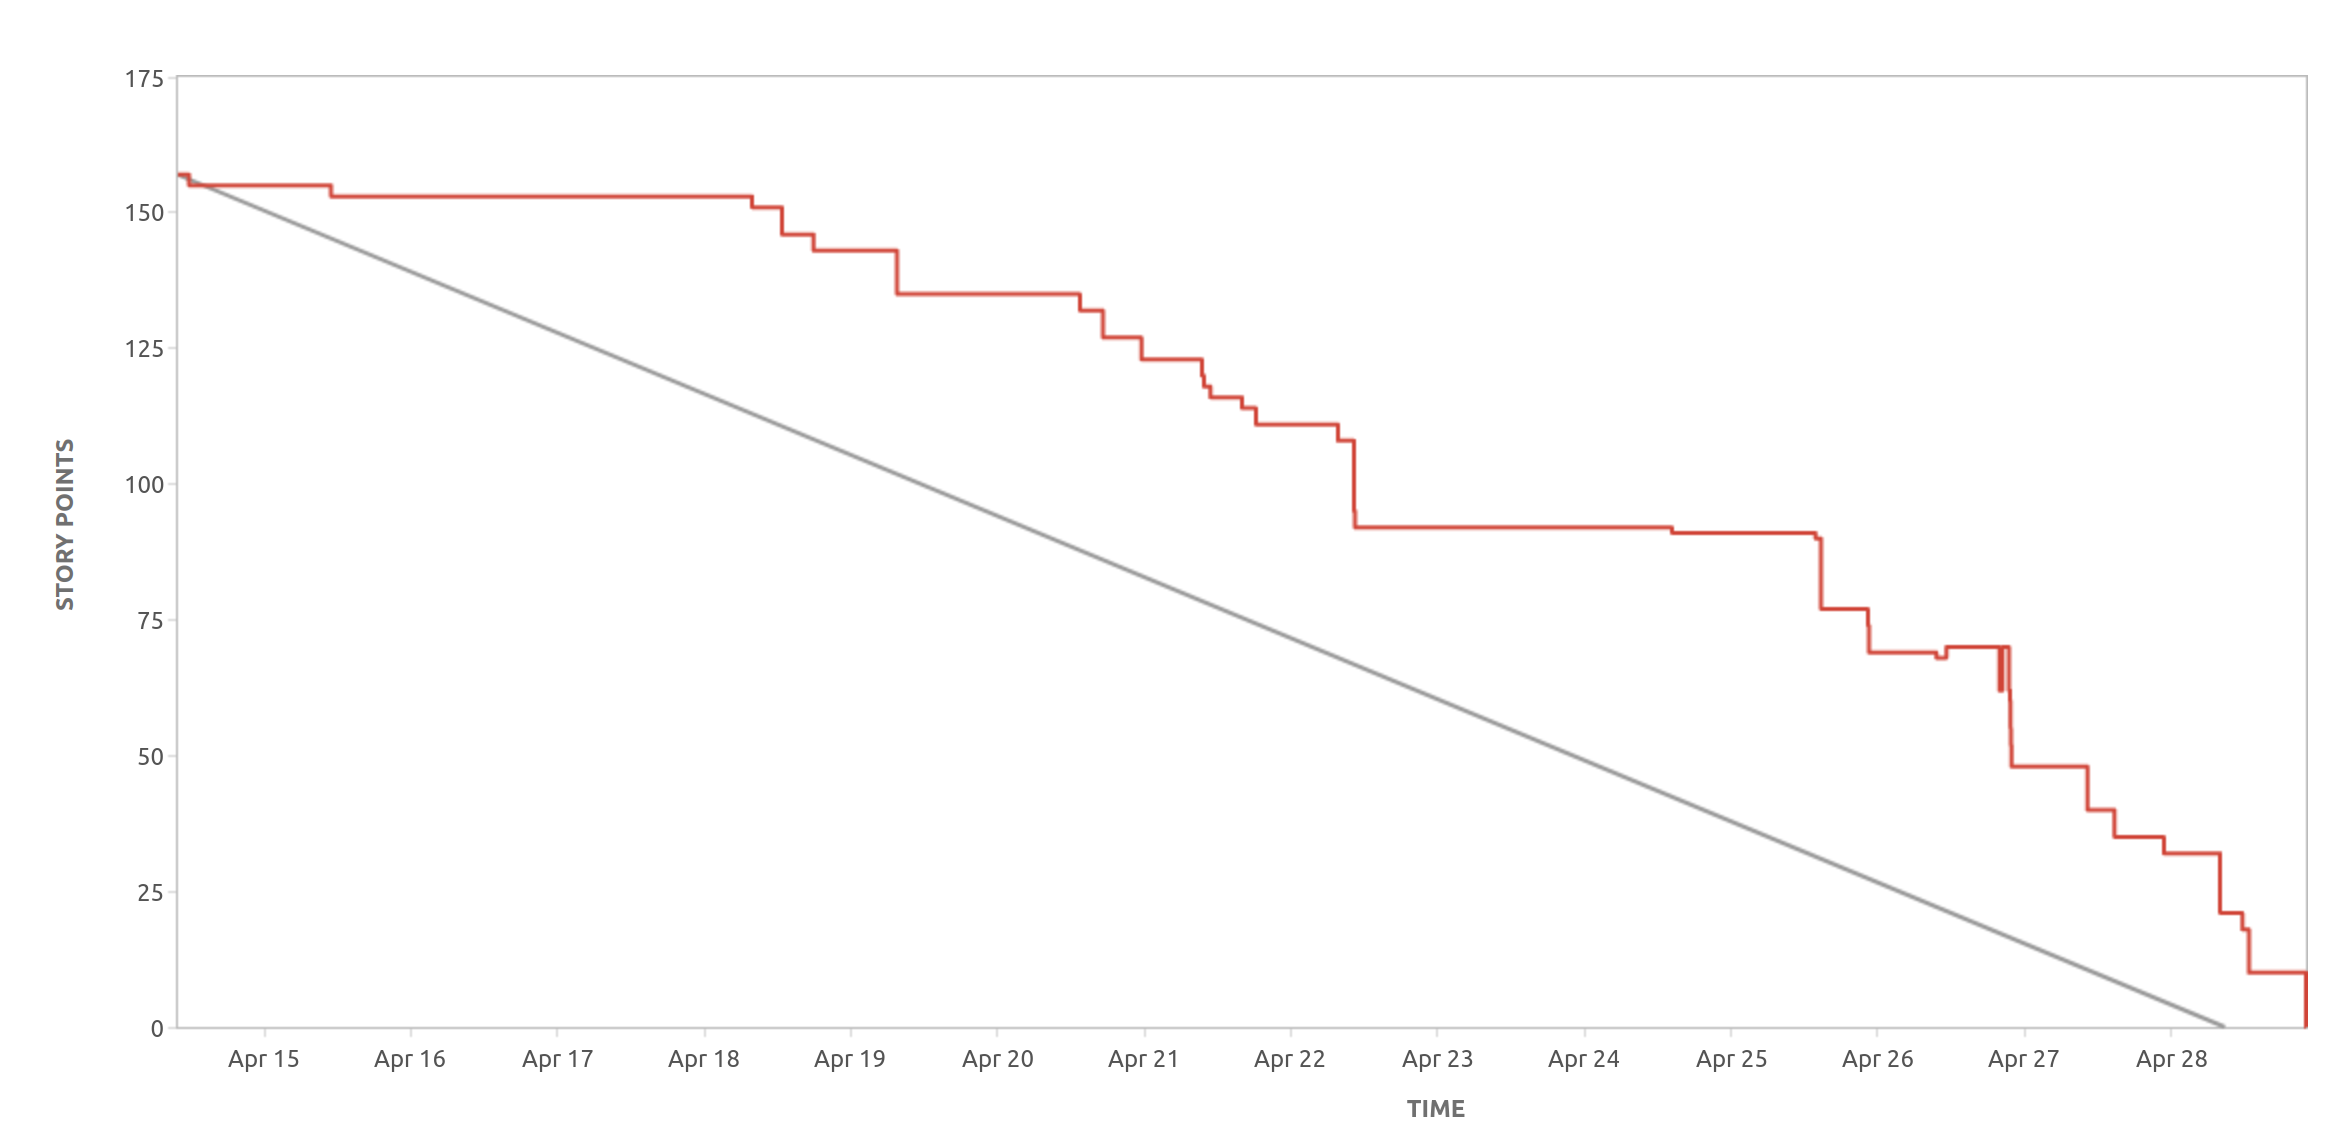
\includegraphics[width=\linewidth]{Skios-Sprint-3-Burndown-Chart.png}
    \caption{Burndown-Chart zu Sprint 3}
    \label{fig:SKIOS-Sprint-3-Burndown}
\end{figure}

\subsection{WIP-Limits}
Zu Anfang des Projektes wurden sehr hohe Initialwerte für die \ac{WIP}-Limits gesetzt.
Das Problem hiermit verdeutlicht sich am besten an der \enquote{Needs Review} Swimlane.
Wie sich in Abbildung \ref{fig:WIP} (dem \ac{WIP}-Chart des Projektes) zeigt, hingen zum Anfang des ersten Sprints ein Großteil der Stories in diesem Status.

\begin{figure}
    \centering
    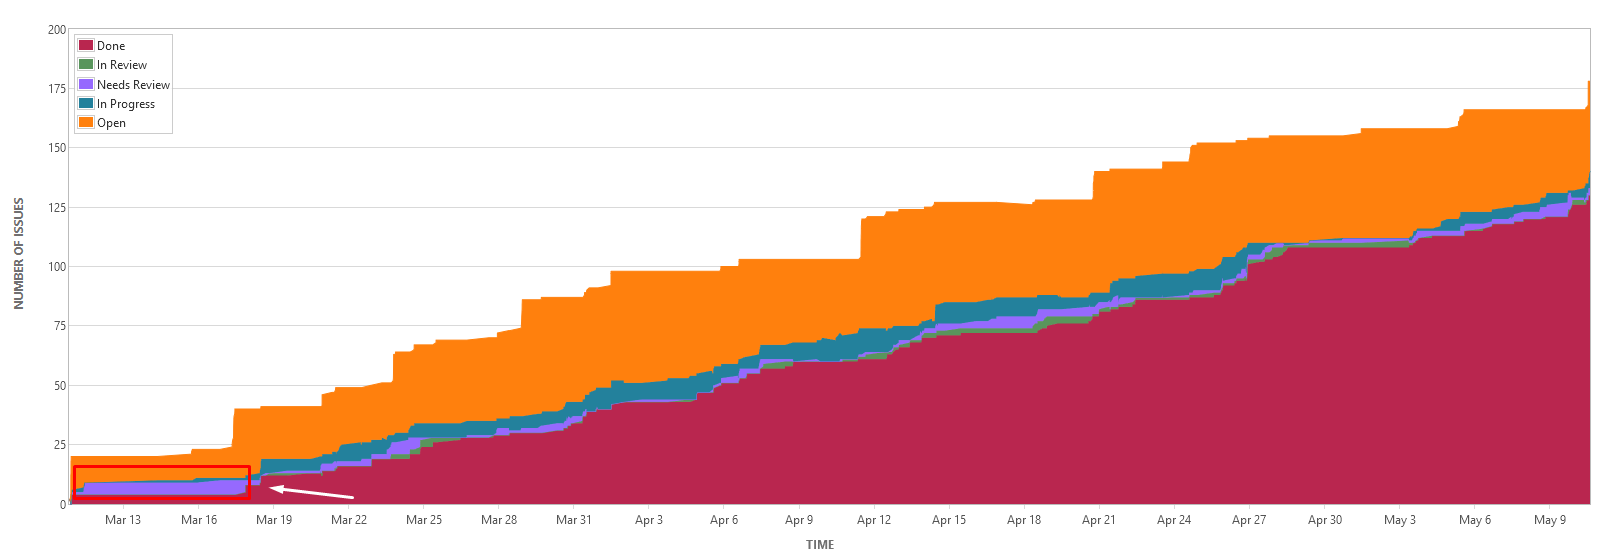
\includegraphics[width=\linewidth]{WIP-Chart.png}
    \caption{WIP Chart des Projektes}
    \label{fig:WIP}
\end{figure}

Als jedoch das \ac{WIP}-Limit dieser Swimlane von 11 auf 4 verringert wurde, ist die Aufhäufung an Tickets dem Team deutlicher geworden.
Im \ac{WIP}-Chart ist ebenfalls eindeutig zu erkennen, dass die Häufung (im Rot umrandeten Bereich) am Anfang sehr prävalent war, sich aber schlagartig zum Zeitpunkt des Einsetzten des Limits zurückgebildet hat (siehe weißer Pfeil).

\subsection{Stories werden von den Service Leads erklärt und nicht vom PO}
Zu Beginn des Projekts ist aufgefallen das die Aufwandsschätzungen für die Tickets 
teilweise sehr ungenau wurden weil das Team die Tickets nicht richtig verstanden hat. 
Deshalb wurde der Prozess dahingehend abgeändert, dass der jeweils zuständige Service 
Lead, ihm zugewiesene, Tickets verstehen und vorstellen muss. So konnte der PO direkt 
anhand der Vorstellung des Tickets erkennen ob verstanden wurde welche Anforderungen 
er an das Ticket hat. Die Veränderung sorgte dafür das Unklarheiten um das Ticket vor
oder während der Vorstellung aufgelöst werden konnten. 

\subsection{Leitlinie für das Erstellen von Tickets}
In den anfänglichen Sprints ist dem Entwicklerteam aufgefallen das die Tickets allein nicht ausreichen 
um zu verstehen was erwartet wird. Um das Erstellen von Tickets zu vereinheitlichen und um sicherzustellen 
das der Entwickler notwendige Information erhält wurde eine Leitlinie entwickelt. 
Diese beschreibt die grobe Einteilung eines Tickets in eine Einleitung, nützliche Informationen für die 
Bearbeitung und Akzeptanzkriterien. Die einzelnen Abschnitte enthalten zudem eine Beschreibung was diese 
enthalten sollen und was sie explizit nicht enthalten sollen. Die Grobstruktur wurde in Jira als Vorlage 
für neue Tickets eingefügt.
Die Leitlinie wurde aktiv umgesetzt und konnte dazu Beitragen das die Entwickler weniger Zeit damit 
verbringen mussten die Erwartungen des Tickets zu recherchieren. 

\subsection{Ausgliederung der Estimations aus den Planungsbesprechungen}

Innerhalb des Ersten Sprintes haben wir sehr viel Zeit für die Kapazitätschätzung benötigt. 
Dies hatte zur Folge, dass im Sprint Planning kaum Zeit für produktive Diskussionen übrig war und mit laufender Dauer die Konzentration für Estimations abnahm.
Daher haben wir beschlossen das Estimation Meeting vom Sprint Planning zu entkoppeln.
So kamen zu den den Bi-Weeklys und ungenutzten Vorlesungsterminen das neue Estimation Meeting hinzu.
Dies führte dazu, dass im Planning Meeting nun genügend Zeit war und die Qualität der Estimations zunahm, was sich in den Burndown-Charts reflektiert.

\section{Erreichte Ziele}
Zusammenfassend lässt sich das Projekt als ein Erfolg betiteln.
Das letztendliche Produkt erfüllt alle must-have requirements und die Delivery des letzten Sprintes stellt einen funktionierenden \ac{MVP} der anfänglich konzipierten RSS-Plattform dar.

Nicht desto trotz ist hervorzuheben, dass nur wenige der Optional-Requirements umgesetzt werden konnten.
Dies lag daran, dass zu Anfang das Projekt von Konzept her zu groß aufgestellt worden ist.
Zwar wäre der Fokus auf Skalierbarkeit und Wartbarkeit außerordentlich wertvoll, falls man mit diesem Projekt nun hätte weiter arbeiten müssen.
Im konstruierten Kontext der Vorlesung hätte man jedoch vermutlich mit einem deutlich eingeschränkteren technischem Aufbau mehr erreichen können.

Zusätzlich ist anzumerken, wie trotz dieser technischen Schwierigkeiten sich das Team in jedem Sprint mehr um mehr verbessert hat.
Besonders an den oben dargestellten Diagrammen ist zu erkennen, dass die Vielzahl an organisatorischen Änderungen im Projekt zu einer spürbaren Verbesserung der Arbeit geführt hat.
Vorallem also an dem Vergleich zwischen dem ersten und letzten Sprints lässt sich das Projekt in Richtung eines sich konstant verbessernden agilen Teams als erfolgreich titulieren.

Zum Zeitpunkt der Abgabe kann die fertige Plattform unter \url{https://skiosa.de/} gefunden werden.

\section{Personenbeiträge}
Die Beiträge der einzelnen Personen sind in Tabelle \ref{tab:person_beitrag} nachzulesen.
Hierbei ist hervorzuheben, dass bei vielen Teammitgliedern Reviews und Fachliche Ausarbeitungen den Großteil deren Mitarbeit dargestellt hat, aber nicht mit in die Story Point Summe miteingeflossen ist. 
Diese Sonstigen Beiträge sind jedoch in der entsprechenden Spalte in der Tabelle nachzulesen

\begin{table}[h]
    \resizebox{\textwidth}{!}{\begin{tabular}{|p{5cm}|p{5cm}|p{5cm}|}
    \hline
    Teammitglied & Summe der Bearbeiteten Story Points & Sonstige Beschreibung der Tätigkeit\\ \hline
    Marcel Alex & 24 & N. A.\\
    Jonas Eppard & 47 & Recomendation und ORM service Lead\\
    Sophie Gösch & 15 & N. A.\\
    Amos Groß & 54 & Projekt Organisation, Ersteller der User Stories und Product Owner\\
    Tim Horlacher & 61 & Architekt und Core Service Lead, hat ein Großteil der Backend/Infra Stories Reviewed\\
    Lukas Huida & 88 & Archtiekt, Organisation der \enquote{bare metal}-infra und server\\
    Theo Krinitz & 19 & N. A.\\
    Sabrina Ladner & 16 & Scrum Master\\
    Simon Morgenstern & 20 & Front-end Service Lead, hat ein Großteil der Frontend Stories Reviewed\\
    Jannik Springer & 41 & Polling Service Lead\\
    \hline
\end{tabular}}
\caption{Tabelle – Personenbeiträge} \label{tab:person_beitrag}
\end{table}
(Eine genaue Beschreibung der Tätigkeiten ist zusätzlich in Kapiteln \ref{team_orga} und \ref{sprints} zu finden)
